\section{Time Rectification and Accuracy}
\label{evaluation-sec-timing}

\begin{figure}[t!]
\begin{center}
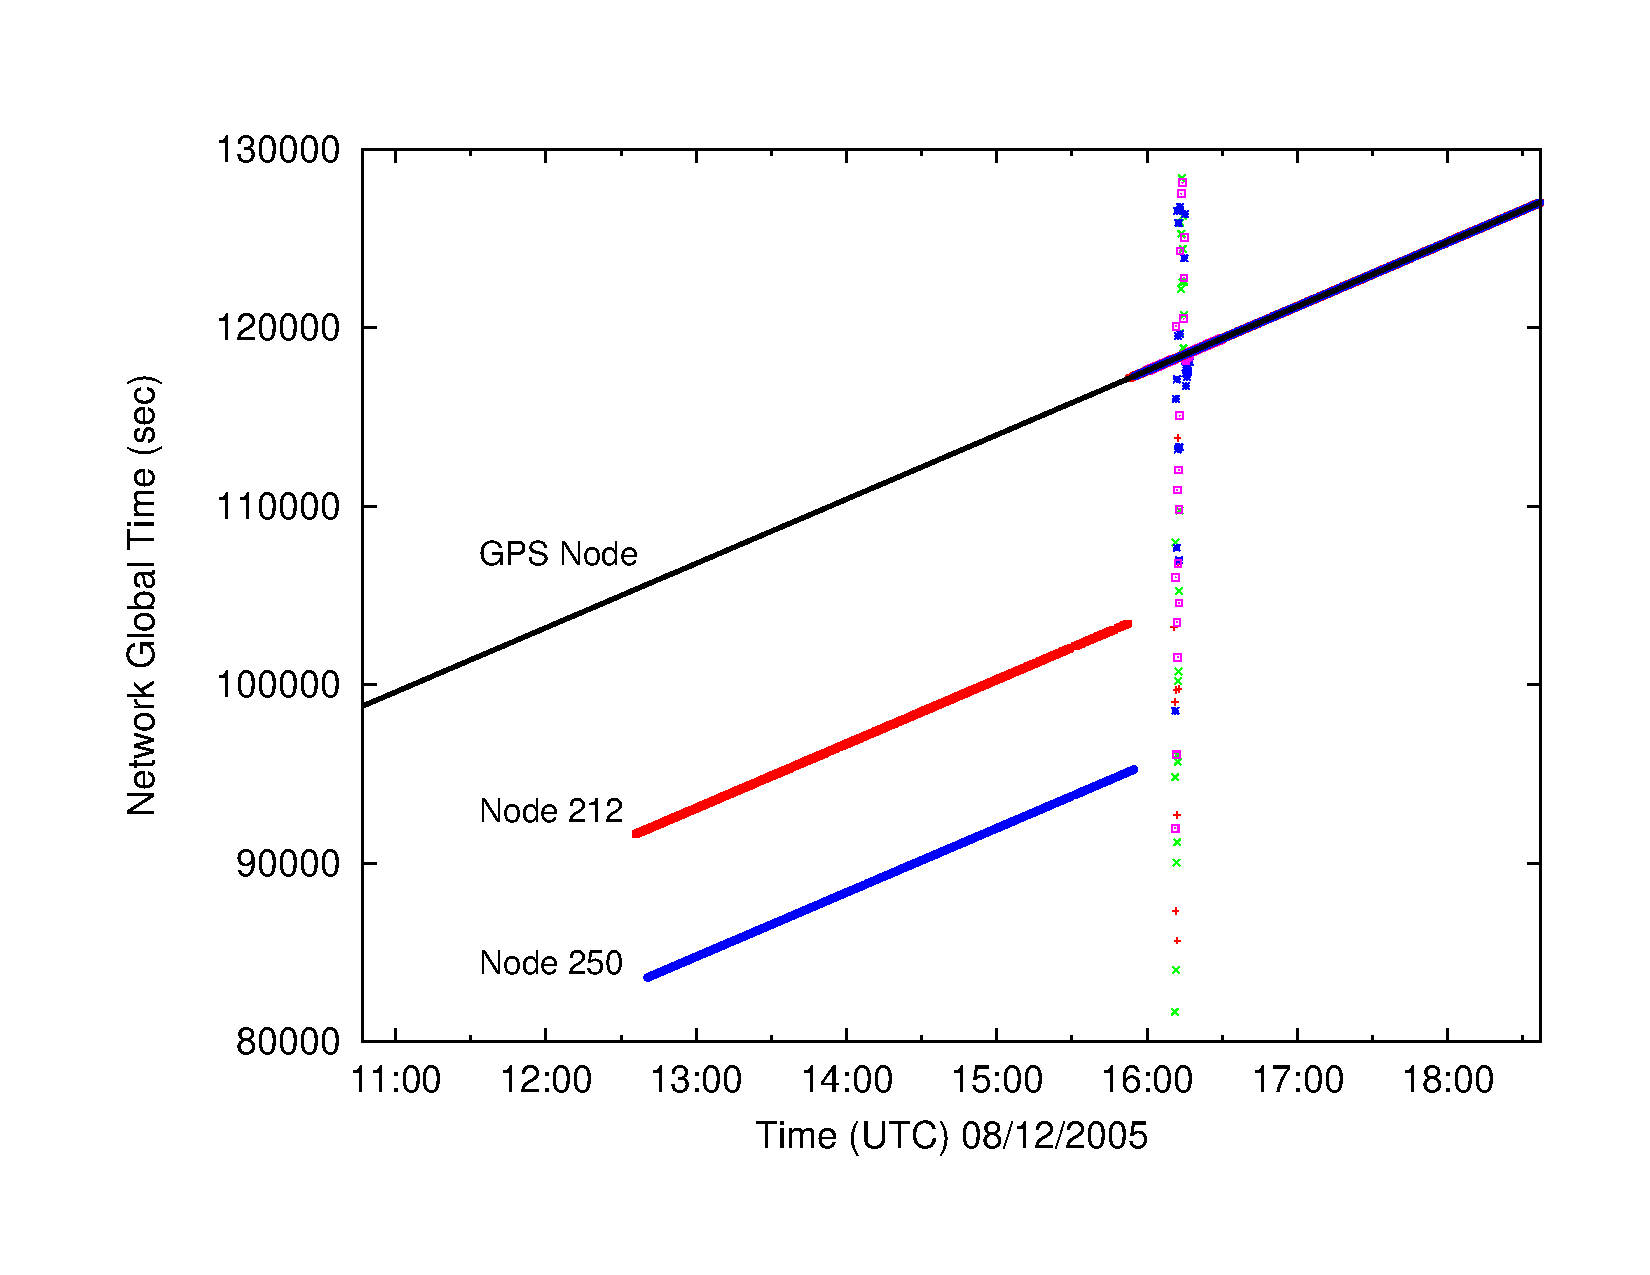
\includegraphics[width=\hsize]{./3-evaluation/figs/globaltimeproblem.pdf}
\end{center} 

\caption{\textbf{Example of observed FTSP instability.} The global time value
reported by sensor nodes and the GPS node is plotted against the time that
the base station received the corresponding status messages. All nodes are
initially synchronized, but starting at 1230 GMT, Nodes~212 and 250 report
incorrect global times for the next 4.5~hours. When the nodes eventually
resynchronize, the global timestamps of other nodes initially experience some
instability.}

\label{evaluation-fig-globaltimeproblem}
\end{figure}

When analyzing seismoacoustic data acquired at volcanoes, accurate timing of
recorded signals is paramount. Studying volcanic source processes
necessitates precisely identifying the arrival time of P-~and S-waves at each
sensor, and correlating signals across the sensor array requires accurately
timestamping each sample.

Ideally, timing should be accurate to within one sample interval, or 10~ms
when sampling at 100~Hz. This requirement is an outgrowth of the prevalent
use of continuous wired data loggers within the seismological community,
which provide highly-accurate timestamps. Since these devices provide such
high-fidelity data, scientists within this community have not had to grapple
with the impacts of larger timing errors or sample reordering. It would be
interesting to discover how these kinds of errors would impact the end-to-end
process of seismological data analysis, but for the purposes of developing
trust in our initial collaboration we chose to try and match the capabilities
of existing instrumentation.

As described earlier, seismologists typically deploy a GPS receiver at each
station. Because GPS receivers are expensive and power hungry, we opted to
use a single GPS receiver and employ a multihop time-synchronization protocol
to establish a global timebase. The protocol worked well in laboratory
experiments. However, it experienced significant failures in the field,
requiring extensive postprocessing of the data to recover accurate timing for
each signal.

Prior internet measurement work has examined similar techniques for error
detection and recovery and produced valuable insights and
advice~\cite{paxson98calibrating,1028824} However, the specific techniques do
not map directly to our application for several reasons. First, they focus
more on error detection and do not address rectification. Second, the sensor
network time synchronization protocols we deployed are new and have goals
distinct from common network time-synchronization protocols. Additionally,
most network measurements can be performed using relative times only, whereas
the scientific requirements of our application required assigning an accurate
absolute timestamp to each collected sample.

In this section, we provide an overview of the time synchronization errors
observed in the field. We then present a novel \textit{time rectification}
technique that allows us to recover accurate timing despite protocol
failures. We evaluate our approach through lab experiments with a known,
ground-truth timebase, and by comparing our signals with signals recorded by
the colocated data loggers.

\subsection{Time Synchronization Architecture}

We chose to use the Flooding Time Synchronization Protocol
(FTSP)~\cite{ftsp}, an existing protocol developed for wireless sensor nodes.
In the original FTSP work~\cite{ftsp}, timing errors of less than 67~$\mu$s
were reported for an 11-hop network of Mica2 nodes. We verified in our
testbed that FTSP provided a 90th-percentile time error of under 2.1~ms in a
5-hop linear network of TMote Sky nodes.

A single MicaZ sensor node was used as the root of the FTSP synchronization
tree. It interfaced to a Garmin GPS receiver and received a 1~Hz interrupt
synchronized to within 1~$\mu$s of the GPS ``pulse per second'' signal.
When the interrupt is raised, the node records the GPS time and corresponding
FTSP global time and sends a short message containing this information to the
base station. Each sensor node runs the FTSP protocol which maintains a
global timebase. Every 10~s, each node records its local time and the
corresponding FTSP global time, sending this information in its status
message to the base station. Finally, as each node records data, the first
sample of each block is marked with the node's local time. After downloading
data from each node following an event, this local time can be used to
recover the time for each sample in the block.

Therefore, we have three relevant timebases: the \textit{local time} at each
node; the \textit{global time} established by the FTSP protocol; and the
\textit{GPS time} recorded by the FTSP root. The information in the nodes'
status messages can be used to map local time to global time, and the
information in the GPS node's status messages can be used to map global time
to GPS-based GMT.

\subsection{FTSP Field Failures}
\label{evaluation-timing-deploymentfailures}

In the absence of failures, this mapping would be a straightforward process.
However, in the field, we noticed that nodes would occasionally lose
synchronization with the rest of the network and report FTSP global times
with significant errors, sometimes exceeding several hours. We suspect that
the sparse deployment conditions at the volcano might have led to different
behavior in the time synchronization protocol than in the lab. For example,
occasional message loss or failure of a neighbor could cause the node's
global time to drift from the rest of the network. However, in lab tests that
constrained the network topology we did not observe these instabilities.

Figure~\ref{evaluation-fig-globaltimeproblem} shows an example of the FTSP
instability observed in the field. The global time reported by two nodes
suddenly jumps off by several hours, and the nodes do not resynchronize until
rebooted 4.5~hours later. It turns out that two bugs conflated to cause this
problem. First, it was discovered that the TinyOS clock driver would
occasionally return bogus local timestamps. This bug was fixed in February
2006, several months after our deployment. Second, FTSP does not check the
validity of synchronization messages, so a node reading an incorrect value
for its local clock can corrupt the state of other nodes, throwing off the
global time calculation.

\begin{figure}[t]
\begin{center}
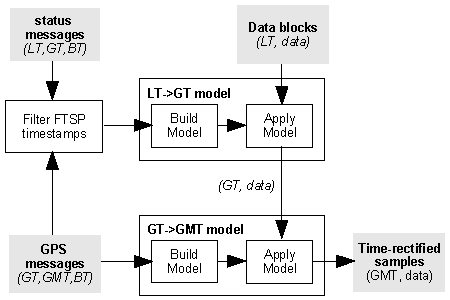
\includegraphics[width=0.8\hsize]{./3-evaluation/figs/rectificationcartoon.pdf}
\end{center}

\caption{\textbf{Time rectification process overview.}}

\label{evaluation-fig-rectificationcartoon}
\end{figure}

The failures of the time synchronization protocol make establishing the
correct GPS-based timestamp for each data sample extremely challenging. Our
\textit{time rectification} approach filters and remaps recorded timestamps
to accurately recover timing despite these failures. The time rectification
process is illustrated in Figure~\ref{evaluation-fig-rectificationcartoon}.
The first step is to \textit{filter} the global timestamps recorded by each
node, discarding bogus data. Second, we build a model mapping the local time
on each node to FTSP-based global time. Third, we use the GPS timestamp
information to build a second model mapping FTSP time to GMT. Finally, both
models are applied to the timestamps recorded in each data block producing a
GMT time for each sample.

\subsection{Timestamp Filtering}
\label{evaluation-subsection-filtering}

We begin by filtering out status messages appearing to contain incorrect
global timestamps. To do this, we correlate global timestamps from each node
against a common reference timebase and reject those that differ by more than
some threshold. For this, we use the base station laptop's local time, which
is \textit{only} used for filtering FTSP timestamps, not for establishing the
correct timing. The filtering process in is many ways similar to prior
work~\cite{paxson98calibrating,1028824} on detecting adjustments in
network-synchronized clocks.

We use the following abbreviations: \textit{LT} is the local time of a node;
\textit{GT} is the FTSP global time; \textit{BT} is the base station's local
time; and \textit{GMT} is the true GMT from the GPS signal. Each GPS status
message logged by the base station consists of the triple \textit{(GT, GMT,
BT)}. We use linear regression on this data to produce a reference timebase
mapping \textit{BT} to \textit{GT}.\footnote{We assume that the global time
reported by the GPS node is always correct; indeed, the definition of
``global time'' is the FTSP time reported by the GPS node. We verified that
the FTSP instability affecting the sensor nodes did not occur on the GPS
node, most likely because the MicaZ uses a different processor that is
unaffected by the clock driver bug.} For each node status message logged by
the laptop \textit{(LT, GT, BT)}, we map \textit{BT} to the expected
$\mathit{GT}_{\mathit{ref}}$ using the reference timebase. If $ \mid
\mathit{GT}_{\mathit{ref}} - \mathit{GT} \mid > \delta$, we discard the
status message from further consideration. We use a threshold of $\delta =
1$~s. Although radio message propagation and delays on the base station can
affect the \textit{BT} for each status message, a small rejection threshold
$\delta$ makes it unlikely that any truly incorrect FTSP timestamps pass the
filter. Indeed, of the 7.8\% of timestamps filtered out, the median
\textit{GT} error was 8.1~hours.
Figure~\ref{evaluation-fig-rectificationexample} shows an example of errant
timestamps being removed.


\subsection{Timestamp Rectification}
\label{evaluation-subsec-timerectification}

\begin{figure}[t]
\begin{center}
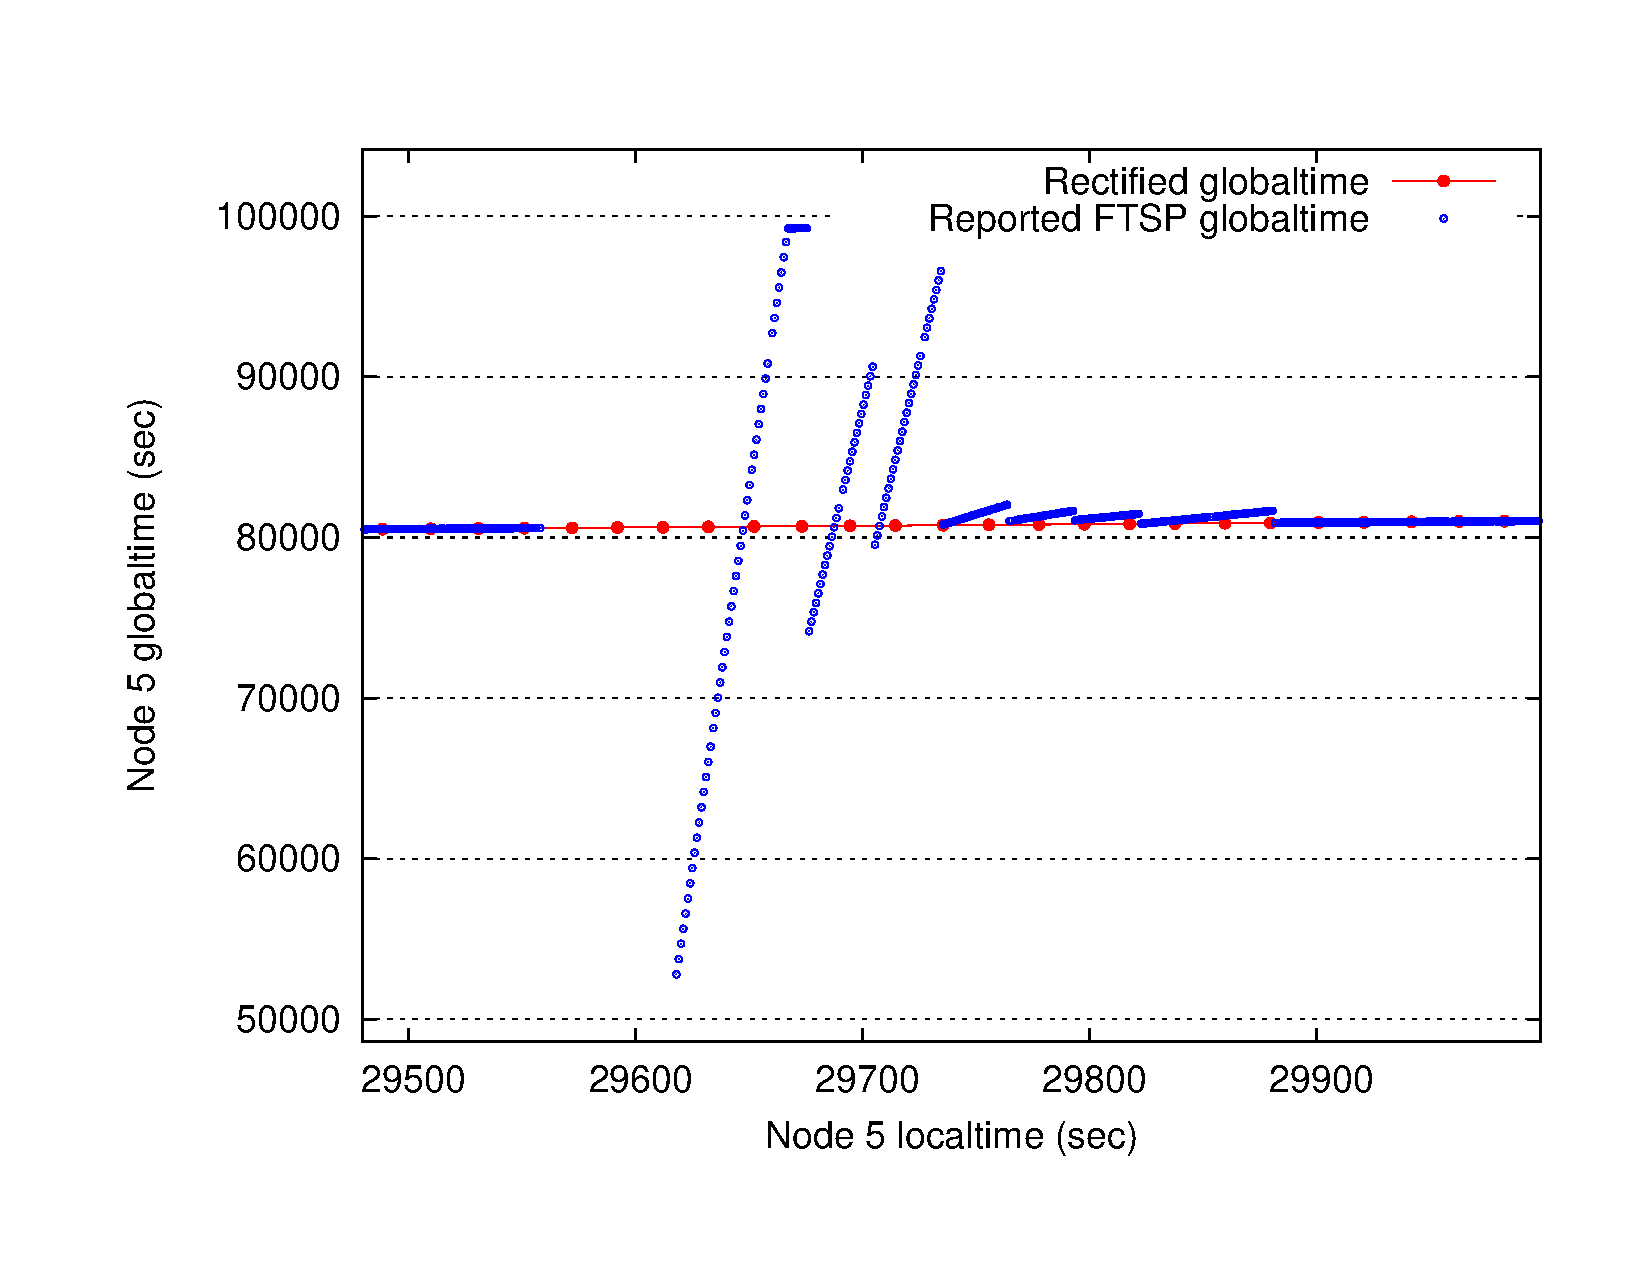
\includegraphics[width=\hsize]{./3-evaluation/figs/rectificationexample.pdf}
\end{center}

\caption{\textbf{Time rectification example.} The raw (LT, GT) pairs
collected from the node show that it experiences a period of FTSP
instability. The time rectification process removes the errant timestamps
creating an accurate mapping between LT and GT created using a linear
regression on the remaining timestamps.}

\label{evaluation-fig-rectificationexample}
\end{figure}

The goal of \textit{time rectification} is to assign a GMT timestamp to each
sample in the recorded data. In order to do so, we build two models: one
mapping a node's local time to global time, and another mapping global time
to GMT. 

From those status messages that pass the filter, we build a piecewise linear
model mapping \textit{LT} to \textit{GT} using a series of linear
regressions. Models are constructed for each node separately, since local
times vary significantly between nodes. Each regression spans up to 5~minutes
of data and we initiate a new regression if the gap between subsequent
\textit{(LT, GT)} pairs exceeds 5~minutes. Each interval must contain at
least two valid status messages to construct the model. We take the
\textit{LT} value stored in each data block and use this model to recover the
corresponding \textit{GT} value.

The next step is to map global time to GMT. Each of the GPS node's status
messages contain a \textit{(GT, GMT)} pair. As above, we build a piecewise
linear model mapping \textit{GT} to \textit{GMT}, and apply this model to the
\textit{GT} values for each data block. Finally, we assign a GMT value to
each sample contained in the block, using linear interpolation between the
GMT values assigned to the first sample in each block. This process makes no
assumptions about sampling rate, which varies slightly from node to node due
to clock drift.

\subsection{Evaluation}
\label{evaluation-timing-postdeployment}

Evaluating this time rectification process has proved difficult, primarily
because we have no ground truth for the timing of the signals recorded in the
field. However, by reproducing the deployment conditions in the lab, we were
able to measure the accuracy of the recovered timing in a controlled setting.
In addition, as described earlier, two GPS-synchronized data loggers were
colocated with our sensor network, providing us the opportunity to directly
compare our time-rectified signals with those recorded by conventional
instrumentation.

Our first validation took place in the lab. Feeding the output of a signal
generator to both a miniature version of our sensor network and to a
Reftek~130 data logger allowed us to directly compare the data between both
systems. The miniature network consisted of a single sensor node, routing
gateway, and GPS receiver node. The same software was used as in the field
deployment. The Reftek~130 logs data to a flash memory card and timestamps
each sample using its own GPS receiver. The Reftek~130 is commonly used in
volcano field studies and its timing accuracy has been extensively validated.

The results showed a consistent 15~ms offset between the time-rectified
signals recorded by the sensor node and the Reftek data logger. We discovered
that this offset was due to delays introduced by the digital filtering
performed by the ADC on our sensor board. Adjusting for this delay resulted
in an indiscernible offset between the sensor node and Reftek signals. While
this experiment does not reproduce the full complexity of our deployed
network, it does serve as a baseline for validation.

In the second lab experiment, we set up a network of 7~sensor nodes in a
6-hop linear topology. The topology is enforced by software, but all nodes
are within radio range of each other, making it possible to stimulate all
nodes simultaneously with a radio message. Each node samples data and sends
status messages using the same software as the field deployment. The FTSP
root node periodically transmits a beacon message. On reception of the
beacon, each node records the FTSP global timestamp of the message reception
time (note that reception of the beacon message is not limited by the
software-induced topology). Because we expect all nodes to receive this
message at the same instant, modulo interrupt latency jitter, we expect the
FTSP time recorded by each node to be nearly identical. The FTSP root also
records the time that the beacon was transmitted, accounting for MAC delay.
The experiment ran for 34~hours, during which time FTSP experienced
instabilities similar to those seen during our deployment.

\begin{table}[t]
\begin{center}
\begin{tabular}{|lll|} \hline & \textbf{Raw error} & \textbf{Rectified error} \\ \hline
\textbf{1 hop}, 50th percentile & 1.52 ms & 1.42 ms \\ 
\textbf{1 hop}, 90th percentile & 9.86 ms & 6.77 ms \\ \hline 
\textbf{6 hops}, 50th percentile & 2.63 ms & 2.18 ms \\ 
\textbf{6 hops}, 90th percentile & 13.5 ms & 6.8 ms \\ \hline 
\end{tabular}
\end{center}

\caption{\textbf{Timestamp errors in a 6-hop lab testbed.} This table shows
the 50th and 90th-percentile timing errors on both the raw FTSP timestamps,
and rectified timestamps.}

\label{evaluation-fig-time-rect-lab}
\end{table}

This allows us to compare the \textit{true} global time of each beacon
message transmission and the \textit{apparent} global time on each receiving
node, both before and after subjecting the data to our time rectification
process. We call the difference between the true and apparent times the
\textit{timestamp error}. Figure~\ref{evaluation-fig-time-rect-lab} shows the
results for nodes one and six hops away from the FTSP root. After
rectification, 99.9\% of the errors for the one-hop node and 93.1\% of the
errors for the six-hop node fall within our 10~ms error envelope.

\subsection{Comparison with Broadband Station}
\label{evaluation-sec-datagroundtruthing}

\begin{figure}[t]
\begin{center}
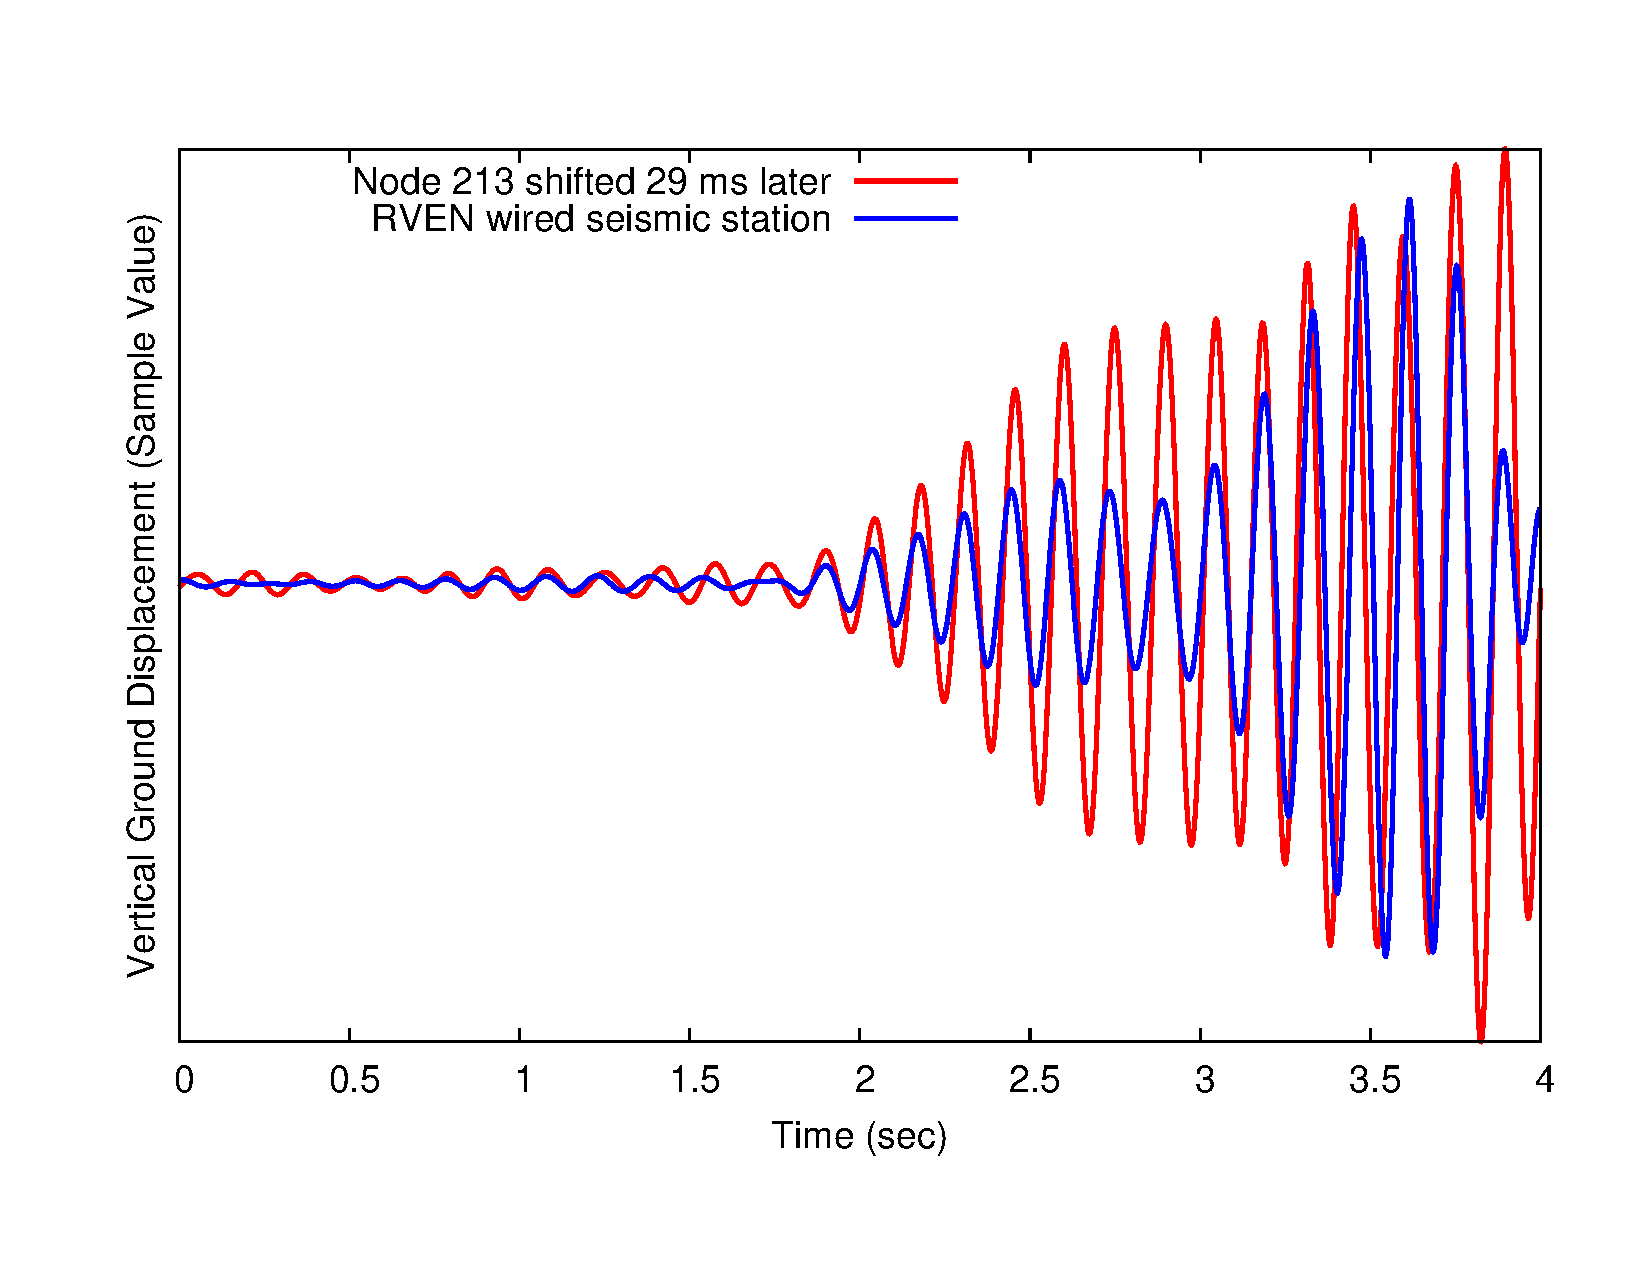
\includegraphics[width=\hsize]{./3-evaluation/figs/broadbandmatch.pdf}
\end{center}

\caption{\textbf{Comparison of RVEN and Node~213 signals.} This figure shows
two seismic waves recorded by sensor node 213 and a broadband seismometer
located 56~m away. After time rectification, a 29~ms time shift produces an
excellent match.}

\label{evaluation-fig-broadbandmatch}
\end{figure}

\begin{figure}[t]
\begin{center}
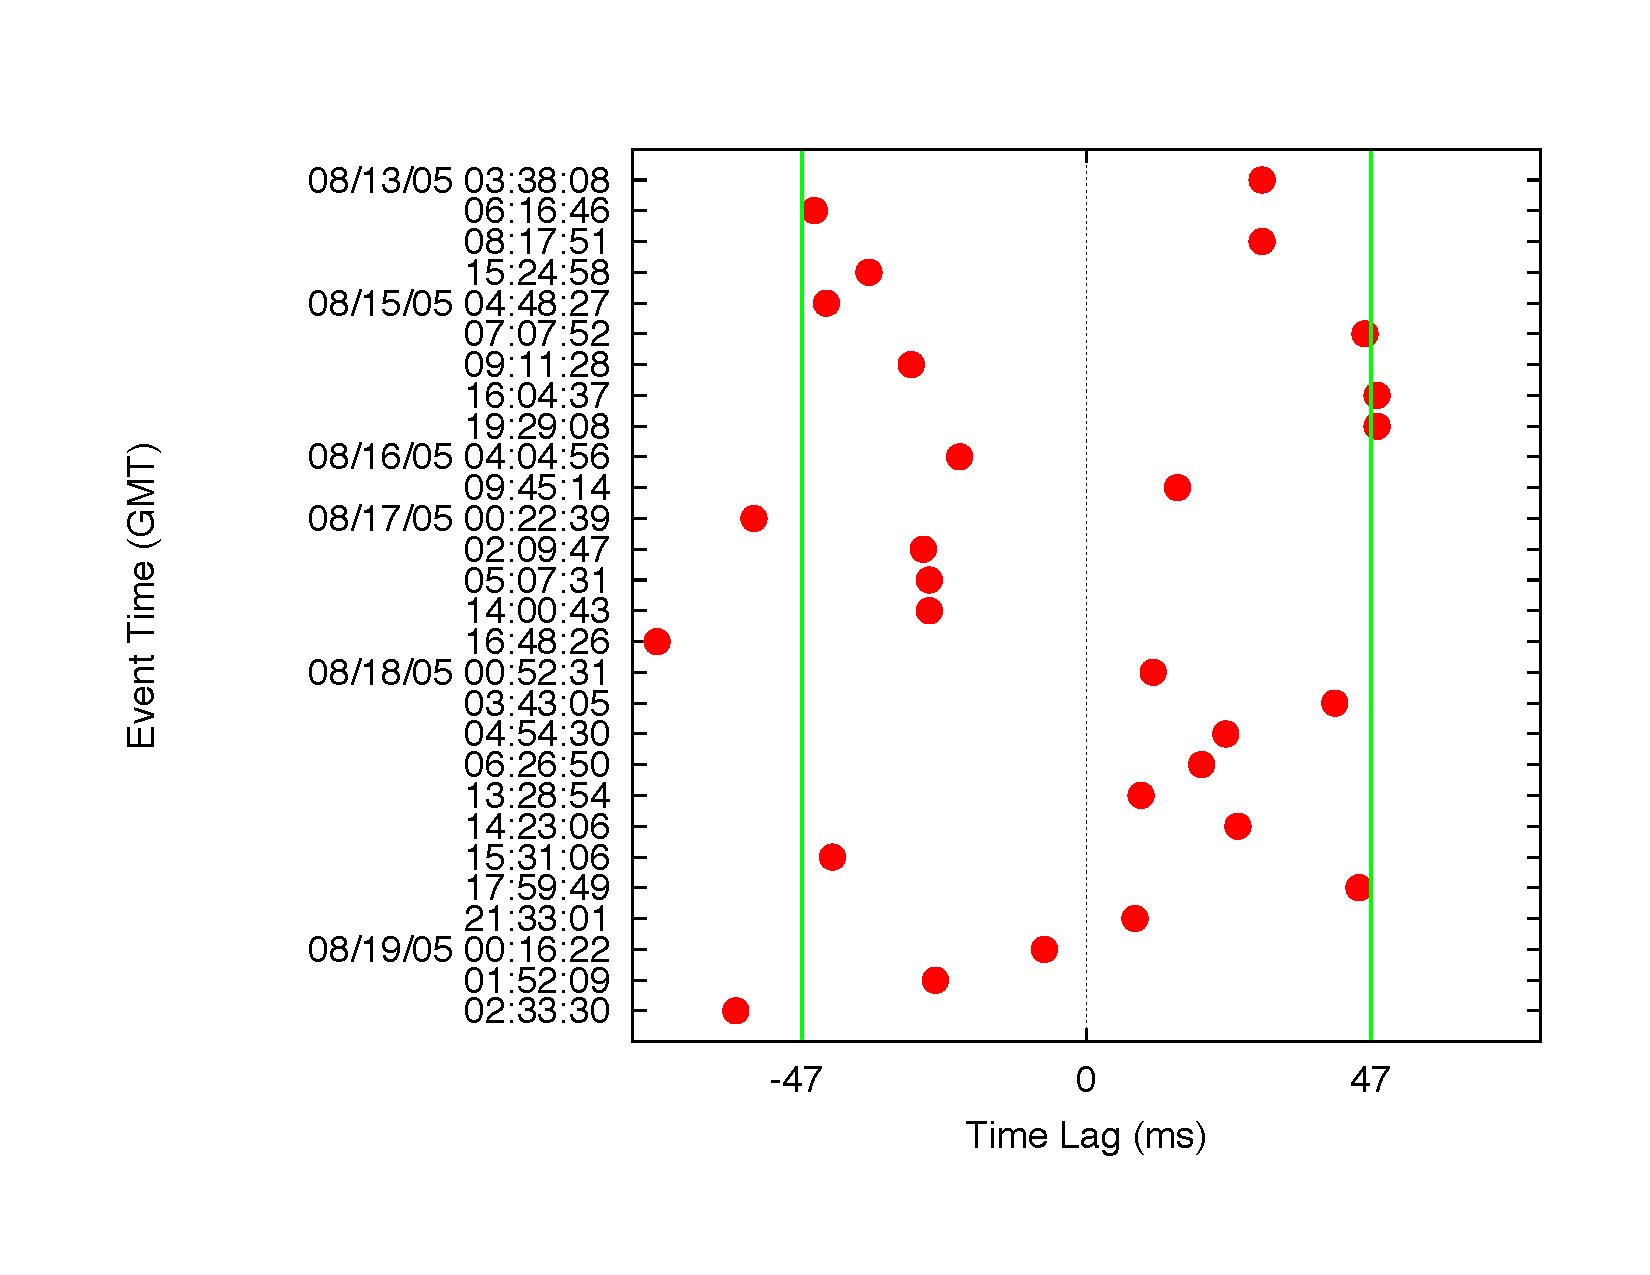
\includegraphics[width=\hsize]{./3-evaluation/figs/timingscatterplot.pdf}
\end{center}

\caption{\textbf{Lag times between Node~213 and RVEN.} The best lag time
between the two stations is shown for 28 events. Most time shifts fall into
the +/-~47~ms window that we would expect given the distance between the two
stations and up to 10~ms of timing error.}

\label{evaluation-fig-timingscatterplot}
\end{figure}


Although time rectification works well in the laboratory, it is also
necessary to evaluate its accuracy on the data collected during the field
deployment. For this purpose, we made use of one of the broadband seismometer
stations colocated with our sensor network. The RVEN (for ``Reventador
vent'') station was located 56~m from sensor Node~213. Given their proximity,
we would expect the seismic waveforms captured by both RVEN and Node~213 to
be well correlated. Some time shift between the two signals would be
expected: a seismic wave passing each station could be as slow as 1.5~km/sec,
so the time lag between the signals could be as high as 37~ms. However, due
to differences in the seismometers and the placement and ground coupling of
the sensors, we would not expect perfectly correlated signals in every case.

We identified 28~events recorded by both RVEN and Node~213. The data for
Node~213 was time rectified as described earlier, and the RVEN data was
timestamped by the Reftek's internal GPS receiver. We applied a bandpass
filter of 6--8~Hz to each signal to reduce sensor-specific artifacts. The
cross-correlation between the signals produces a set of of \textit{lag times}
indicating possible time shifts between the two signals. Due to the periodic
nature of the signals, this results in several lag times at multiples of the
dominant signal period. For each lag time, we visually inspected how well the
time-shifted signals overlapped and picked the best match by hand.

Figure~\ref{evaluation-fig-broadbandmatch} shows an example of this process
that demonstrates excellent correlation between the RVEN and Node~213 signals
with a 29~ms time shift. Figure~\ref{evaluation-fig-timingscatterplot} shows
a scatterplot of the best lag times for all~28~events. Of these, only
5~events fall outside of a $+/-$~47~ms window defined by the distance between
the stations ($+/-$~37~ms) and our acceptable sampling error (10~ms). We have
high confidence that our time rectification process was able to recover
accurate timing despite failures of the FTSP protocol.
